\section{Back-end}


\subsection{Interfaccia REST}

Ad ogni richiesta il server può rispondere con un messaggio di errore nel formato \glossario{JSON} e inviato con un codice \glossario{HTTP} della tipologia 4xx o 5xx. 
Il formato \glossario{JSON} del messaggio di errore sarà:
\begin{lstlisting}
{ 
  "code": [codice numerico dell'errore],
  "message": [descrizione testuale dell'errore],
  "data": [eventuali dati aggiuntivi sull'errore]
}
\end{lstlisting}
Di seguito sono elencate le risorse REST associate al tipo di metodo che è possibile richiedere su esse e i permessi richiesti per poter effettuare la richiesta. \\
I tipi di permessi possibili sono: 
\begin{itemize}
\item \textbf{Utente}: questa risorsa può essere richiesta da qualsiasi tipo di utente;
\item \textbf{Utente Autenticato}: questa risorsa può essere richiesta solo dagli utenti autenticati a \glossario{MaaP};
\item \textbf{Admin}: tale risorsa può essere richiesta solo da utenti con livello Admin.
\end{itemize}

\begin{center}
	\def\arraystretch{1.5}
	\bgroup
	\begin{longtable}{| p{9cm} | p{1.5cm} | p{4cm} |}
	\hline 
	\textbf{\emph{/login}} & \textbf{POST} & \textbf{Utente} \\ \hline
	\multicolumn{3}{|c|} {Crea una nuova sessione associata all'utente, corrisponde al login.} \\ \specialrule{1pt}{1pt}{1pt}
	
	\multicolumn{3}{c} {} \\ \hline
	
	%\specialrule{1pt}{1pt}{1pt} 
	
	\textbf{\emph{/logout}} & \textbf{DELETE} & \textbf{Utente Autenticato} \\ \hline
	\multicolumn{3}{|c|} {Elimina la sessione utente, corrisponde al logout. }  \\ \specialrule{1pt}{1pt}{1pt}
	
	\multicolumn{3}{c} {} \\ \hline
	
	\textbf{\emph{/profile}} & \textbf{GET} & \textbf{Utente Autenticato} \\ \hline
	\multicolumn{3}{|c|} {Restituisce i dati relativi all'utente. }  \\ \hline
	\textbf{\emph{/profile}} & \textbf{PUT} & \textbf{Utente Autenticato} \\ \hline
	\multicolumn{3}{|c|} { Modifica i dati utente. }  \\ \specialrule{1pt}{1pt}{1pt}
	
	\multicolumn{3}{c} {} \\ \hline
	
	\textbf{\emph{/password/lost}} & \textbf{POST} & \textbf{Utente} \\ \hline
	\multicolumn{3}{|c|} {Effettua la richiesta di recupero password. }  \\ \specialrule{1pt}{1pt}{1pt}
	
	\multicolumn{3}{c} {} \\ \hline
	
	\textbf{\emph{/password/reset}} & \textbf{PUT} & \textbf{Utente} \\ \hline
	\multicolumn{3}{|c|} {Effettua la richiesta di modifica della password utente. }  \\ \specialrule{1pt}{1pt}{1pt}
	
	\multicolumn{3}{c} {} \\ \hline
	
	\textbf{\emph{/users}} & \textbf{GET} & \textbf{Admin} \\ \hline
	\multicolumn{3}{|c|} {Restituisce la lista di tutti gli utenti. }  \\ \hline
	\textbf{\emph{/users}} & \textbf{POST} & \textbf{Admin} \\ \hline
	\multicolumn{3}{|c|} {Effettua la richiesta di creazione di un nuovo utente. }  \\ \specialrule{1pt}{1pt}{1pt}
	
	\multicolumn{3}{c} {} \\ \hline
	
	\textbf{\emph{/users/$\{$user id$\}$}} & \textbf{GET} & \textbf{Admin} \\ \hline
	\multicolumn{3}{|c|} {Restituisce i dati corrispondenti all'utente con id $\{$user id$\}$. }  \\ \hline
	\textbf{\emph{/users/$\{$user id$\}$}} & \textbf{PUT} & \textbf{Admin} \\ \hline
	\multicolumn{3}{|c|} {Modifica i dati dell'utente con id $\{$user id$\}$. }  \\ \hline
	\textbf{\emph{/users/$\{$user id$\}$}} & \textbf{DELETE} & \textbf{Admin} \\ \hline
	\multicolumn{3}{|c|} {Elimina l'utente con id $\{$user id$\}$. }  \\ \specialrule{1pt}{1pt}{1pt}
	
	\multicolumn{3}{c} {} \\ \hline
	
	\textbf{\emph{/collection}} & \textbf{GET} & \textbf{Utente Autenticato} \\ \hline
	\multicolumn{3}{|c|} {Restituisce la lista delle collection. }  \\ \specialrule{1pt}{1pt}{1pt}
	
	\multicolumn{3}{c} {} \\ \hline
	
	\textbf{\emph{/collection/$\{$collection name$\}$} } & \textbf{GET} & \textbf{Utente Autenticato} \\ \hline
	\multicolumn{3}{|c|} {Restituisce la lista di document della collection $\{$collection name$\}$.}  \\ \specialrule{1pt}{1pt}{1pt}
	
	\multicolumn{3}{c} {} \\ \hline
	
	\textbf{\emph{/collection/$\{$collection name$\}$/$\{$document id$\}$}  } & \textbf{GET} & \textbf{Utente Autenticato} \\ \hline
	\multicolumn{3}{|c|} {Restituisce la lista di attributi del Document $\{$document id$\}$ appartenente alla collection $\{$collection name$\}$}  \\ \hline
	\textbf{\emph{/collection/$\{$collection name$\}$/$\{$document id$\}$} } & \textbf{PUT} & \textbf{Admin} \\ \hline
	\multicolumn{3}{|c|} {Modifica il document $\{$document id$\}$. }  \\ \hline
	\textbf{\emph{\emph{/collection/$\{$collection name$\}$/$\{$document id$\}$} }} & \textbf{DELETE} & \textbf{Admin} \\
	\hline
	\multicolumn{3}{|c|} {Elimina il document con id $\{$document id$\}$. }  \\ \specialrule{1pt}{1pt}{1pt}
	
	\multicolumn{3}{c} {} \\ \hline
	
	\textbf{\emph{/action/$\{$action name$\}$/$\{$collection name$\}$}} & \textbf{PUT} & \textbf{Utente Autenticato} \\ \hline
	\multicolumn{3}{|c|} {Esegue l'azione $\{$action name$\}$ sulla Collection $\{$collection name$\}$.}  \\ 
	\specialrule{1pt}{1pt}{1pt}
	
	\multicolumn{3}{c} {} \\ \hline
	
	\textbf{\emph{/action/$\{$action name$\}$/$\{$collection name$\}$/$\{$document id$\}$}} & \textbf{PUT} & \textbf{Utente Autenticato} \\ \hline
	\multicolumn{3}{|c|} {Esegue l'azione $\{$action name$\}$ sul Document $\{$document name$\}$ della Collection 
	$\{$collection name$\}$.}  \\ 
	\specialrule{1pt}{1pt}{1pt}

	
\end{longtable}
	  \egroup
\end{center}

\subsection{Diagramma dei package}

\subsection{Diagrammi gestione richieste}
Nel diagramma della gestione richieste viene mostrata l'iterazione tra server e middleware, quest'ultimi possono essere diversi, tra cui i middleware utilizzati da Express:
\begin{itemize}
\item{basicAuth()}: Middleware per l'autenticazione HTTP di base. Questo middleware causa il rifiuto delle richieste con userneme e password non corretti con stato HTTP "401 Unauthorized".
\item{bodyParser()}: Middleware che analizza una richiesta di tipo JSON o di tipo www-form-encoded.
\item{cookieParser()}: Middleware che analizza il campo header dei Cookie.
\item{cookieSession()}: Middleware per la gestione di sessioni utente basate su cookies.
\item{router()}: Middleware in cui Express gestisce le richieste registrate ai metodi GET,POST etc, , ovvero mappa azioni diverse a richieste http diverse, sia in termini di url che in termini di metodi http.
\item{static()}: Middleware per la gestione dei contenuti statici.
\item{error-handling}: middleware per la gestione degli errori. La risposta di tale middleware è di tipo arbitrario, può essere risposta una pagina HTML di errore, un semplice messaggio o una stringa JSON.
\item{passport}: middleware per Node.js utilizzati per implementare l'autenticazione in maniera semplice e veloce, vengono utilizzati:
	\begin{itemize}
	\item{passport.initialize()}: middleware utilizzato per l'inizializzazione di Passport.
	\item{passport.session()}:  middleware che permette di memorizzare i record della sessione utente per mantenerne lo stato di
	login. 
	\end{itemize}
\item{notFoundMiddleware}: un middleware da noi scritto per gestire le richieste che non vengono gestite (errore client 4xx).
\item{errorMiddleware}: middleware da noi scritto per gestire gli errori sollevati da uno dei precedenti middleware (errore server
500)
\end{itemize}
La richiesta arriva al server il quale va a prendere il prossimo \glossario{middleware}, inviandogli come parametri la richiesta, la risposta e next che innesca la chiamata per passare il controllo al prossimo \glossario{middleware}.  \\
In caso di errore, l'ultimo middleware manderà un next(error) ed il server aggiungerà un parametro a quelli sopra citati con l'informazione dell'errore stesso e passerà il controllo al primo gestore dell'errore e non al successivo \glossario{middleware}. \\
Un \glossario{middleware} può rispondere con un return() ed in questo caso ..... %TODO \\

\begin{figure}[H]
	\begin{center} 
		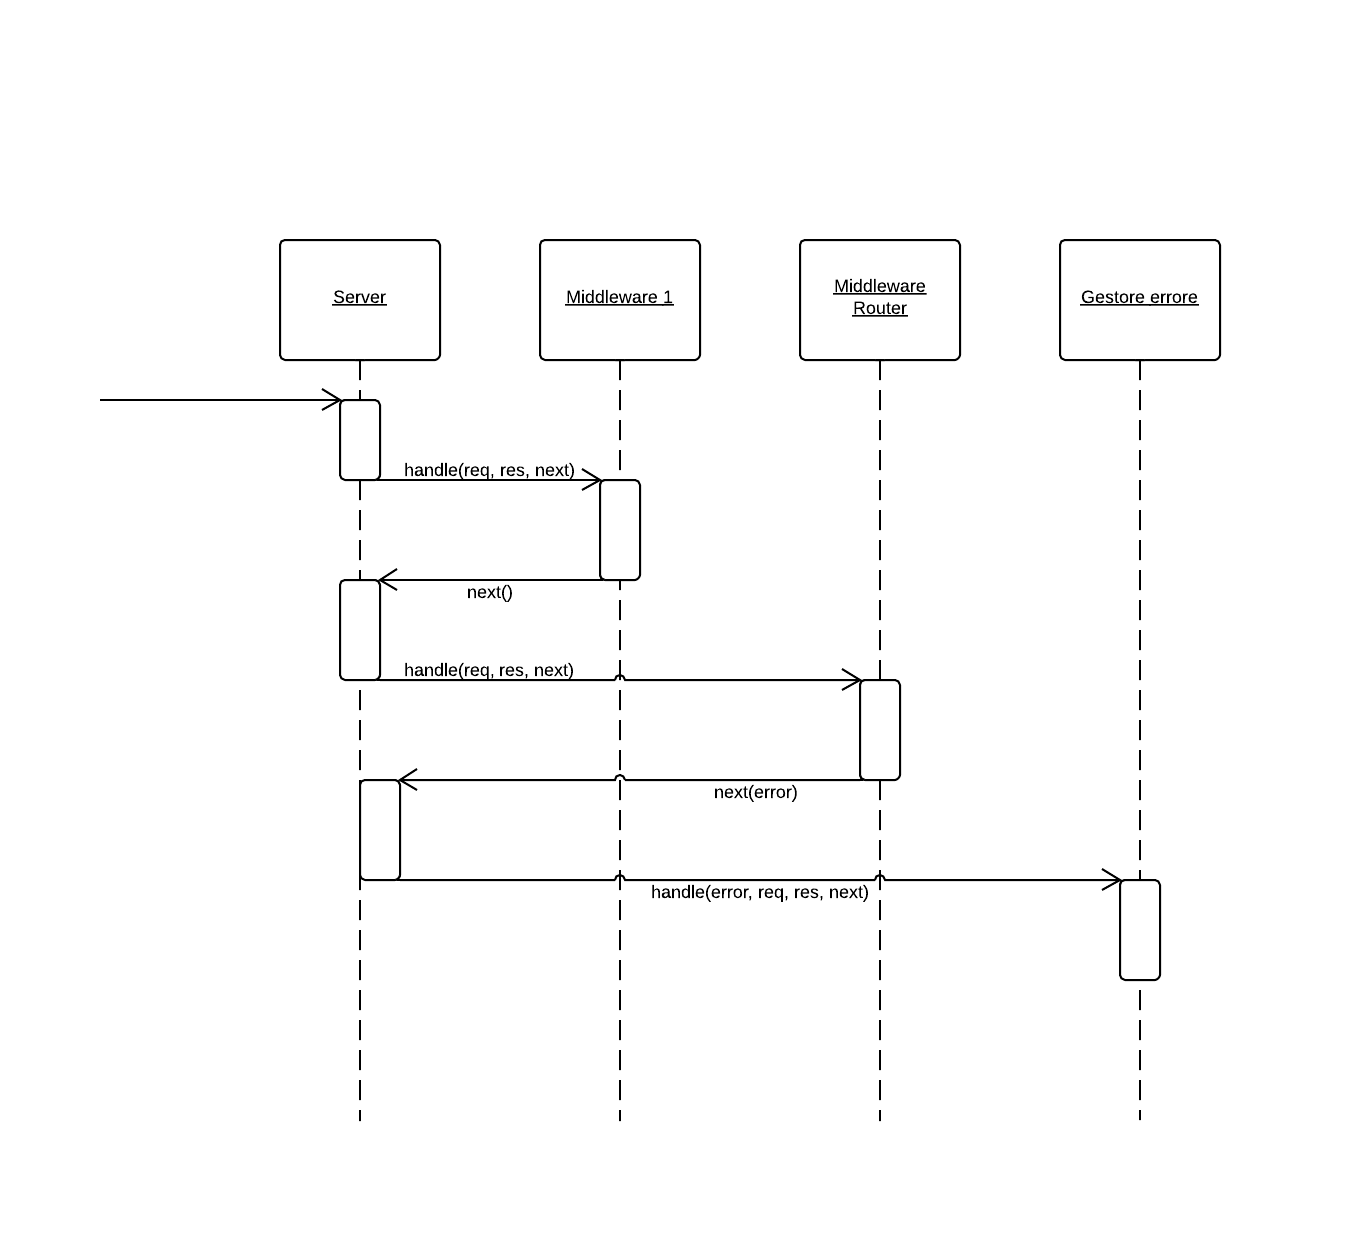
\includegraphics[scale=0.30]{scenari/Diagramma Gestione Richiesta.png}  
		\caption{Diagramma Gestione Richiesta}
	\end{center} 
\end{figure} 

Nel seguente diagramma viene mostrato il comportamento di routing, dove si intende che ogni controllore ha associato un'espressione regolare che specifica su quali richieste agisce.
\begin{figure}[H]
	\begin{center} 
		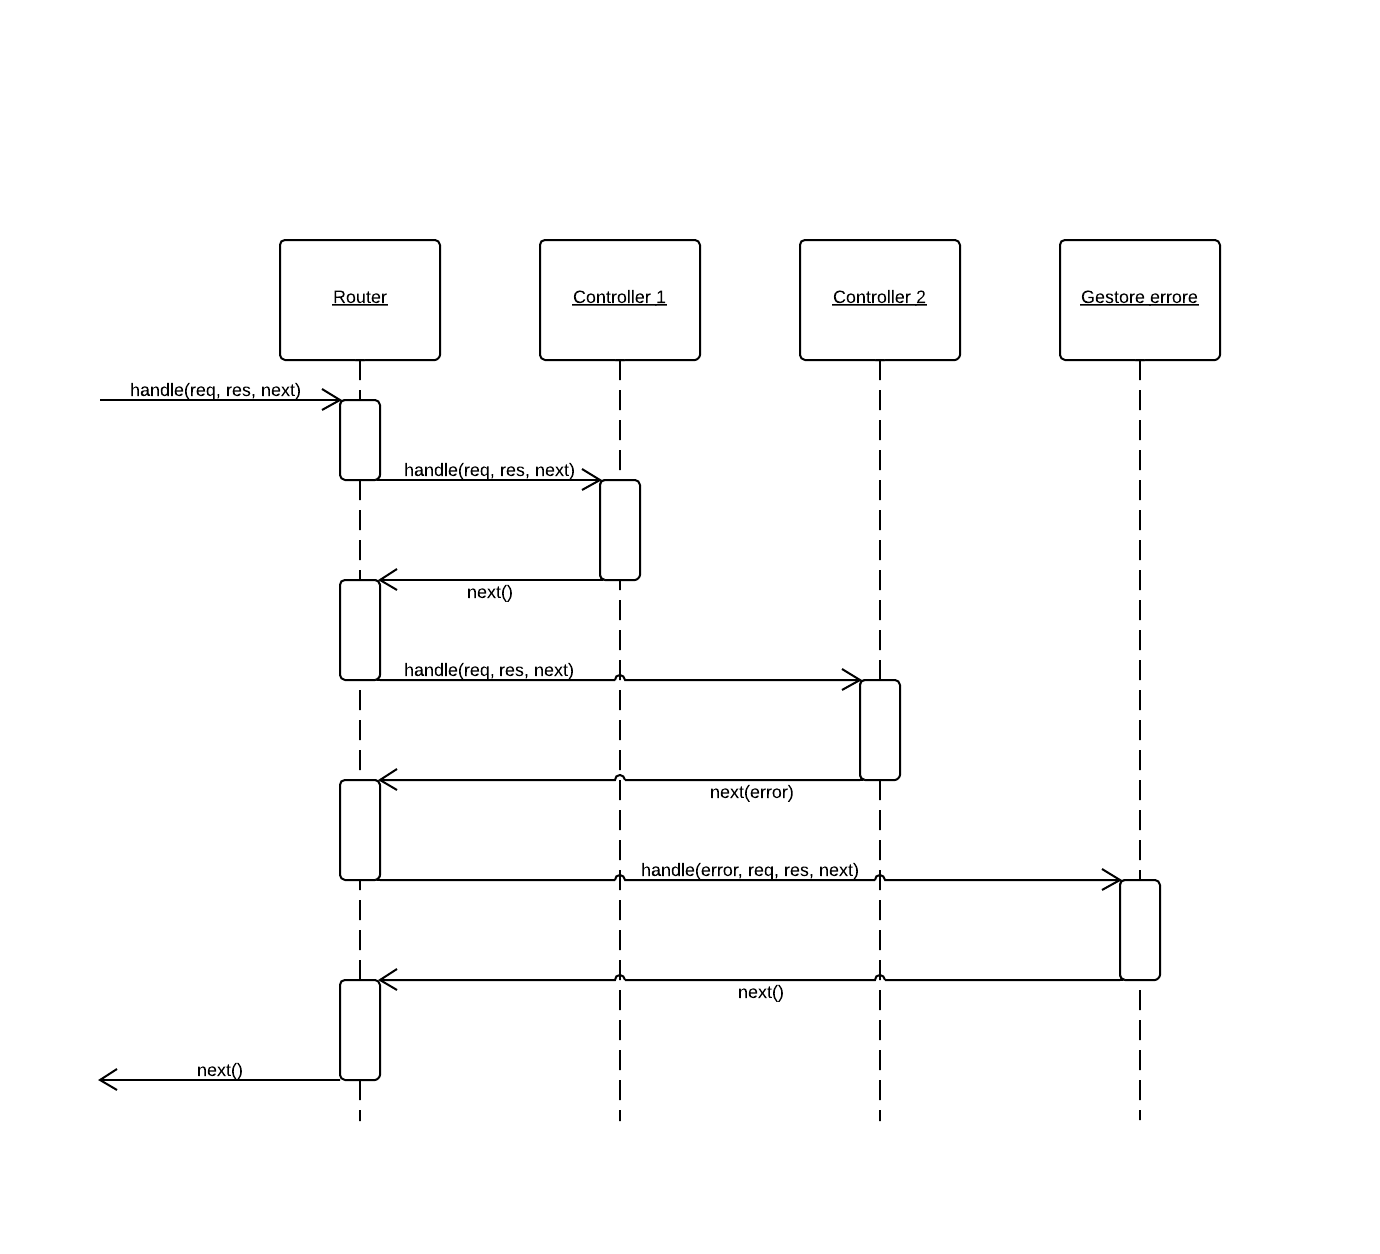
\includegraphics[scale=0.30]{scenari/Diagramma Routing Richiesta.png} 
		\caption{Diagramma Routing Richiesta}
	\end{center} 
\end{figure}

\subsection{Scenari}

\subsubsection{Fallimento vincolo ``utente autenticato''}
Descrizione scenario, dire che si riferisce a tutti quelli che avranno un requireLogged
Diagramma: PassportLocal requireLogged ERROR

\subsubsection{Fallimento vincolo ``utente non autenticato''}
Descrizione scenario, dire che si riferisce a tutti quelli che avranno un requireNotLogged
Diagramma: PassportLocal requireNotLogged ERROR

\subsubsection{Fallimento vincolo ``utente admin''}
Descrizione scenario, dire che si riferisce a tutti quelli che avranno un requireAdmin
Diagramma: PassportLocal requireAdmin ERROR

\subsubsection{Login POST}
Descrizione scenario
Precondizione: non fallisce il requireNotLogged
Diagramma: Login POST

\subsubsection{Logout DELETE}
Descrizione scenario
Precondizione: non fallisce il requireLogged
Diagramma: Logout DELETE

\subsubsection{Profile GET}
Descrizione scenario
Precondizione: non fallisce il requireLogged
Diagramma: Profile GET
Controller: requireLogged, ProfileController->getProfile()

\subsubsection{Profile PUT}
Descrizione scenario, dire che come precondizione non fallisce il requireLogged
Diagramma: Profile PUT
Controller: requireLogged, ProfileController->editProfile()

\subsubsection{Password Lost POST}
Descrizione scenario, dire che come precondizione non fallisce il requireNotLogged
Diagramma: Password Lost POST
Controller: requireNotLogged, ForgotController->requirePasswordReset()

\subsubsection{Password Reset PUT}
Descrizione scenario, dire che come precondizione non fallisce il requireNotLogged
Diagramma: Password Reset PUT
Controller: requireNotLogged, ForgotController->makePasswordReset()

\subsubsection{Users GET}
Descrizione scenario, dire che come precondizione non falliscono i controlli
Diagramma: Users GET
Controller: requireLogged, requireAdmin, UserController->getUsers()

\subsubsection{Users POST}
Descrizione scenario, dire che come precondizione non falliscono i controlli
Diagramma: Users POST
Controller: requireLogged, requireAdmin, UserController->createUser()

\subsubsection{Users Id GET}
Descrizione scenario, dire che come precondizione non falliscono i controlli
Diagramma: Users Id GET
Controller: requireLogged, requireAdmin, UserController->getUser(id)

\subsubsection{Users Id PUT}
Descrizione scenario, dire che come precondizione non falliscono i controlli
Diagramma: Users Id PUT
Controller: requireLogged, requireAdmin, UserController->editUser(id)
Lo UserController può restituire un errore se si cerca di modificare un superadmin o se si cerca di modificare il proprio ruolo.

\subsubsection{Users Id DELETE}
Descrizione scenario, dire che come precondizione non falliscono i controlli
Diagramma: Users Id DELETE
Controller: requireLogged, requireAdmin, UserController->deleteUser(id)
Lo UserController può restituire un errore se si cerca di modificare un superadmin o se si cerca di modificare il proprio ruolo.

\subsubsection{Collection GET}
Descrizione scenario, dire che come precondizione non falliscono i controlli
Diagramma: Collection GET
Controller: requireLogged, CollectionController->listCollections()

\subsubsection{Collection Name GET}
Descrizione scenario, dire che come precondizione non falliscono i controlli
Diagramma: Collection Name GET
Controller: requireLogged, CollectionController->indexPage(collection)

\subsubsection{Collection Name Document GET}
Descrizione scenario, dire che come precondizione non falliscono i controlli
Diagramma: Collection Name Document GET
Controller: requireLogged, CollectionController->showPage(collection)

\subsubsection{Collection Name Document PUT}
Descrizione scenario, dire che come precondizione non falliscono i controlli
Diagramma: Collection Name Document PUT
Controller: requireLogged, requireAdmin, CollectionController->editDocument(collection, document)

\subsubsection{Collection Name Document DELETE}
Descrizione scenario, dire che come precondizione non falliscono i controlli
Diagramma: Collection Name document DELETE
Controller: requireLogged, requireAdmin, CollectionController->deleteDocument(collection, document)

\subsubsection{Action Name Collection PUT}
Descrizione scenario, dire che come precondizione non falliscono i controlli
Diagramma: Collection Name document DELETE
Controller: requireLogged, requireAdmin, CollectionController->collectionAction(action, collection)

\subsubsection{Action Name Collection Document PUT}
Descrizione scenario, dire che come precondizione non falliscono i controlli
Diagramma: Collection Name document DELETE
Controller: requireLogged, requireAdmin, CollectionController->documentAction(action, collection, document)
